%%%%%%%%%%%%%%%%%%%%%%%%%%%%%%%%%%%%%%%%%%%%%%%%%%%%%%%%%%%%%%%%%%%%%%%%
%%%%%%%%%%%%%%%%%%%%%%%%%%%%%%%%%%%%%%%%%%%%%%%%%%%%%%%%%%%%%%%%%%%%%%%%
\section{Methods}
\label{chapter:methods}
Three methods will be used to estimate the orientation and compared against each other, OPPR, MBPE and GRAT. The first was described in \ref{cha2:opprandsphere}, MBPE will be presented in this section and as for GRAT some alterations to what was explained on section \ref{eppppp} will be presented. As well as that, the algorithms GRAT and MBPE will use the fact that, in the particular geometry of this system the translation will be derived from the baseline constraint.
\subsection{Translation derivation}
\label{rignreg}
Because the current eye prototype is a coupled system, the translation can be obtained through the knowledge of the rotation and the baseline length associated. This length is defined as the distance from the center of the camera's sensor to the center of rotation, as shown on Figure \ref{cha3:detori:translation}.
\begin{figure}[ht]
	\centering
	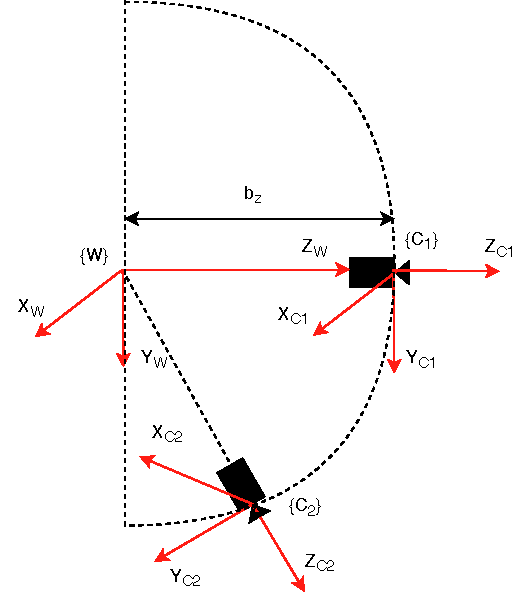
\includegraphics[width=0.3\textwidth]{images/transf.pdf}
	\caption[Translation derivation]{The rotation and the baseline length define the translation. ${W}$ is the world reference frame centered on the rotation center, ${C_1}$ is the reference frame of the camera in the first position and ${C_2}$ is its frame on the second position, after rotating. $b_z$ is the baseline length on the Z (torsional) axis.}
	\label{cha3:detori:translation}
\end{figure}

The translation can be derived from using frame to frame transformations\footnote{Consult Chapter 2 of Introduction to ROBOTICS mechanics and control \cite{robotics} on Spatial descriptions and transformations}. Having the world reference frame, ${W}$, set at the center of rotation, the transformation from the world to the first position of the camera, ${C_1}$, is
\begin{equation}
^{C_1}T_{W} = \begin{bmatrix}
I & -\mathbf{b}\\ 
\mathbf{0} & 1
\end{bmatrix},
\end{equation} 
where $\bf b$ is the baseline length expressed in each axis as $\mathbf{b} = [b_X \ b_Y \ b_Z]$. 
The transformation from the world reference frame to the second position of the camera, ${C_2}$, is
\begin{equation}
^{C_2}T_{W} = \begin{bmatrix}
R & -\mathbf{b}\\ 
\mathbf{0} & 1
\end{bmatrix},
\end{equation}\\
where $R$ is the rotation.
Hence, the transformation from the first position of the camera to the second can be obtained as
\begin{equation}
\begin{split}
^{C_2}T_{C_1} = ^{C_2}T_W  \ ^WT_{C_1} =\\
\begin{bmatrix}
R & -\mathbf{b}\\ 
\mathbf{0} & 1
\end{bmatrix}
\begin{bmatrix}
I & \mathbf{b}\\ 
\mathbf{0} & 1
\end{bmatrix}
=
\begin{bmatrix}
R & R\mathbf{b}-\mathbf{b}\\ 
\mathbf{0} & 1
\end{bmatrix}
\end{split}.
\end{equation}
And finally, the translation ends up as
\begin{equation}
\mathbf{t}(R, \mathbf{b}) = R\mathbf{b}-\mathbf{b} = (R-I)\mathbf{b}.
\end{equation}

\subsection{Minimization of the backprojection error (MBPE)}

This algorithm tries to minimize the error between the real image points, $\mathbf{\tilde{m}_1}$ and $\mathbf{\tilde{m}_2}$, and its back projections, $\mathbf{\tilde{m}^r_1}$ and $\mathbf{\tilde{m}^r_2}$, estimating the variables $R$ and $\mathbf{t}$ directly instead of using the fundamental matrix, $F$, as an intermediate like it was described on section \ref{eppppp}. Three parameters are enough to define the rotation (see section \ref{cha2:represent}) and consequently the translation, $\mathbf{t}(R, \mathbf{b})$, as is dependent.\\
The back projections of the points can be obtained by
\begin{align}
\label{cha2:epipolar:shitshit1}
\lambda_2 \mathbf{\tilde{m}^r_2} = K [ R \ \mathbf{t} ] K^{-1} \lambda_1 \mathbf{\tilde{m}_1}\\
\label{cha2:epipolar:shitshit2}
\lambda_1 \mathbf{\tilde{m}^r_1} =  K [ R^{T} \ -R^{T}\mathbf{t} ] K^{-1}  \lambda_2 \mathbf{\tilde{m}_2},
\end{align}
where $K$ are the known intrinsic parameters of the camera and $\lambda_1$ and $\lambda_2$, the depth of the corresponding 3D points, is unknown. Therefore, it has to be estimated for each point, making a total of $3+n$ variables to estimate in the minimization.
The cost function to this algorithm is then
\begin{equation}
\label{fiorenfe}
\begin{split}
   	\min_{\mathbf{\theta}, \lambda^r_{11}, ..., \lambda^r_{1n}} \sum^n_{i=1} [(u^r_{1i}-u_{1i})^2  + (v^r_{1i}-v_{1i})^2 +\\ (u^r_{2i}-u_{2i})^2 + (v^r_{2i}-v_{2i})^2] 
\end{split}
\end{equation}
where $[u_{1i} \ v_{1i}] = \mathbf{m_{1i}}$ are the pixel points in the image before rotating, $[u_{2i} \ v_{2i}] = \mathbf{m_{2i}}$ are the pixel points after rotating, $[u_{1i}^r \ v_{1i}^r] = \mathbf{m_{1i}^r}$ and $[u_{2i}^r \ v_{2i}^r] = \mathbf{m_{2i}^r}$ are its corresponding back projections, $\lambda^r_{11}, ..., \lambda^r_{1n}$ are the estimated depths and $\mathbf{\theta} = [\theta_Z \ \theta_Y \ \theta_X]$ are Euler angles used to determine the rotation.

The back projections should be obtained by
\begin{align*}
	\mathbf{\tilde{m}_{1}^r} = \frac{KR(\mathbf{ \theta})^T(\lambda_{2}^r K^{-1}\mathbf{\tilde{m}_2}) - R(\mathbf{ \theta})^T \mathbf{t}(R(\mathbf{ \theta}), \mathbf{b}))}{\lambda_{1}^r}\\
	\mathbf{\tilde{m}_{2}^r} = \frac{KR(\mathbf{ \theta})(\lambda_{1}^r K^{-1}\mathbf{\tilde{m}_1}) + \mathbf{t}(R(\mathbf{ \theta}), \mathbf{b}))}{\lambda_{2}^r}.
\end{align*} 

In order to start running the algorithm it's necessary to give it initialization parameters, $\lambda_{1}^r$ and $\lambda_{2}^r$ can be acquired from the projection of the image points in a 3D sphere, explained in section \ref{cha2:opprandsphere}, and the Euler angles, $\mathbf{\theta}$, can be given by OPPR as it's a fast and light-weight approximation.

\subsection{Gradient-Based Tecnhique (GRAT)}
\label{fjeopfe}
Regarding what was said on section \ref{eppppp}, instead of obtaining $R$ and $\mathbf{t}$ through the factorization of the fundamental matrix, $F$, they can be estimated rather than estimating $F$. Furthermore, given that $\mathbf{t}$ depends on $R$, like before only 3 parameters have to be estimated. 
This constraint can be used in combination with the most promising epipolar method explained on section \ref{eppppp}, GRAT. A similar approach is taken by Vasconcelos F. et al \cite{vasconcelos}
to calibrate a camera using multiple sets of pairwise correspondences, in section ``8.2 Bundle Adjustment". 
The cost function for this algorithm is then
\begin{align}
\min_\mathbf{\theta} \sum_i \frac{ (\mathbf{\widetilde{\mathbf{m}}_{2i}}^T F \widetilde{\mathbf{m}}_{1i})^2}{\sigma_i^2} \ \text{with}\\
F = K^{-T} [\mathbf{t}]_\times R(\mathbf{ \theta}) K^{-1} \ \text{and}\\
\label{dopewnrvno}
\sigma_i^2 =  [l_{{e1i}_x}^2 + l_{{e1i}_y}^2 + l_{{e2i}_x}^2 + l_{{e2i}_y}^2],
\end{align}
where $\sigma_i^2$ is the variance, $l_{e1i} = F\widetilde{\mathbf{m}}_{2}$ and $l_{e2i} = F\widetilde{\mathbf{m}}_{1}$ are the epipolar lines for each point $i$, $\mathbf{\theta}$ are the Euler angles and $R(\mathbf{ \theta})$ is a rotation matrix obtained through \ref{rrr}. Once again, the initialization of $\mathbf{ \theta}$ can be done using OPPR.\\

As opposed to MBPE, in GRAT the depths of the 3D points are not necessary. The explicit representation of 3D points is avoided by minimizing the perpendicular distances between point correspondences and their epipolar lines \cite{vasconcelos} \cite{bundle}.

\section{Implementation}
\label{chapter:implementation}

\begin{figure}[ht]
	\centering
	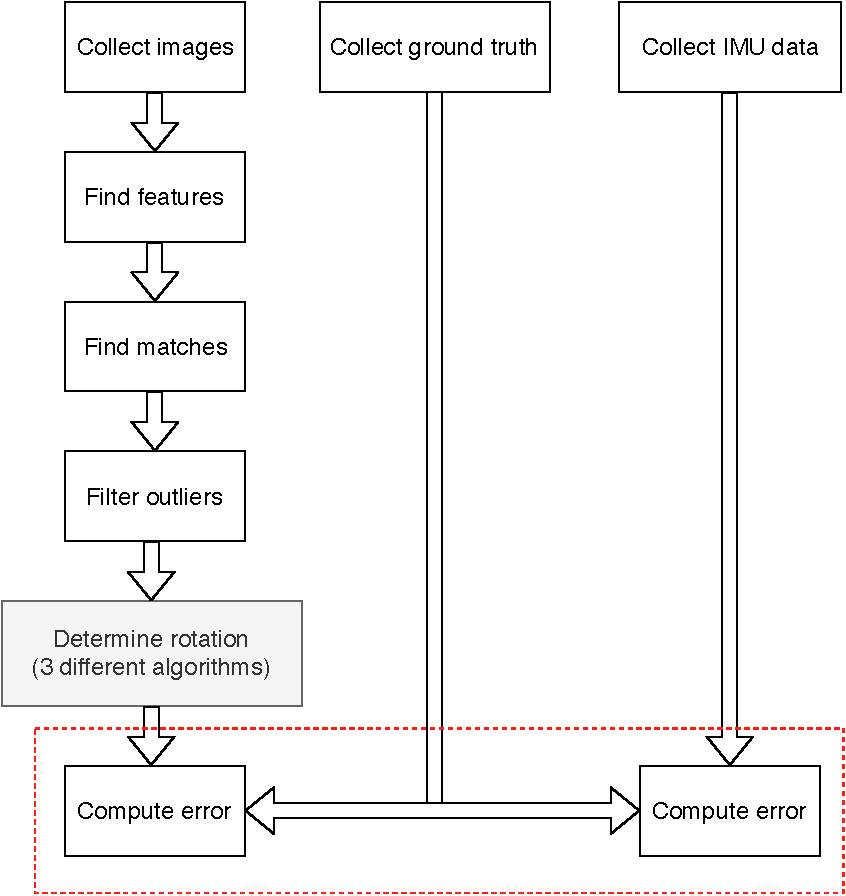
\includegraphics[width=0.5\textwidth]{images/approach.pdf}
	\caption[Flow Diagram]{Flow Diagram. The RGB camera collects two images, before and after rotation. In each image, features are detected and matched between them. Some matches might be false or have too much noise, so they are filtered out. Using the matches information, the executed rotation is determined using an estimation algorithm. The three algorithms are tested. Finally, the estimated rotation is compared against the ground truth. The IMU's orientation output is also compared against the ground truth to evaluate its performance in relation to the camera.}
	\label{cha3:methodology:approach}
\end{figure}
Figure \ref{cha3:methodology:approach} shows the flow of the procedures that determine the eye rotation. It specifies what is needed to determine the rotation of the camera for real data sets. However, in order to evaluate the three algorithms in a controlled environment, a simulator was implemented which generates image point matches/correspondences with known rotations. These points may contain additive Gaussian noise, or even false matches to test the performance of the outlier filtering and the resilience of the estimator. 

Both the simulator and the procedures to deal with real data were implemented in Matlab\footnote{\href{https://www.mathworks.com/products/matlab.html}{https://www.mathworks.com/products/matlab.html}} and can be found in the thesis github repository\footnote{\href{https://github.com/Mrrvm/Orient/tree/master/Matlab}{https://github.com/Mrrvm/Orient/tree/master/Matlab}}. A C++ library was also created to deal with the data on the real system for convenience and computational speed, and can also be found at the repository\footnote{\href{https://github.com/Mrrvm/Orient/tree/master/C++}{https://github.com/Mrrvm/Orient/tree/master/C++}}.

\subsection{Real system Procedures} 

\subsubsection{Eye prototype setup}
Figure \ref{cha4:sec3:eyescheme} shows the current eye prototype  The distance from the center of rotation to the camera, defined previously as baseline length, is $[0 \ 0 \ 53.7] \pm 3 \ mm $. This setup was fixed $5 \ m$ away from furthest object in the scene.
\begin{figure}[ht]
	\centering
	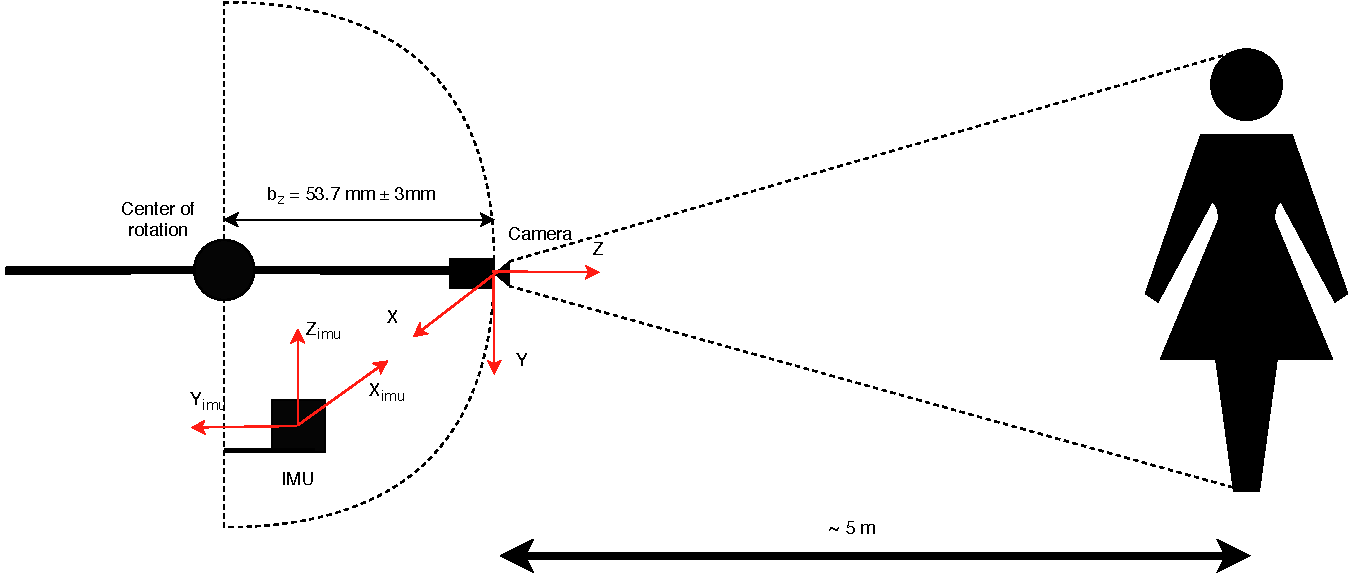
\includegraphics[width=0.5\textwidth]{images/eyescheme.pdf}
	\caption[Eye prototype scheme used on the experiments]{Eye prototype scheme used on the experiments. The camera is displaced from the center of rotation by $b_z$ }
	\label{cha4:sec3:eyescheme}
\end{figure}

\subsubsection{Collect images}
The camera was calibrated and the images were collected using an uEye LE USB3 camera in grayscale before and after a certain rotation.

\subsubsection{Collect ground truth}
Using the same camera in the same positions, two images were taken with a chessboard on the scene, which is used to determine the ground truth through its regular pattern. This images are then loaded into a Matlab algorithm\footnote{\href{https://www.mathworks.com/help/vision/ref/detectcheckerboardpoints.html}{https://www.mathworks.com/help/vision/ref/detectcheckerboardpoints.html}} that determines the ground truth. It's important to note that there is error associated to the ground truth that can heavily affect the outcome of the experiments.	 

\subsubsection{Feature detection and matching}
It is necessary to gather corresponding features in consecutive images taken before and after a rotation, and to use an algorithm to estimate the orientation using those features. The latter, also referred to as keypoints or interest points, are spatial locations of an image that ``stand out", allowing them to be identifiable. These points should be such that even after rotating, translating, shrinking or distorting the image, they can be found. There exist a multitude of algorithms that can do the job. Salahat E. and Qasaimeh M. in 2017 \cite{featsift}, presents an overview on the recent algorithms, comparing them in terms of distinctiveness, locality, quantity, accuracy, efficiency, repeatability, invariance and robustness. The analysis in that article suggests that Maximally stable extremal regions (MSER) and Scale Invariant Feature Transform (SIFT) algorithms enhance performance on computational complexity, accuracy and execution time. From the scale and rotation invariant algorithms, Speeded Up Robust Features (SURF), proved to be faster than SIFT, although not as robust. Because SURF is faster and more accessible due to patenting concerns regarding SIFT, it will be be used on this work.

Regarding the matching of feature descriptors, one of the most common search algorithms used, that will also be used here, is the Nearest Neighbor Search. Fast Library for Approximate Nearest Neighbour (FLANN) \cite{flann} provides a library for performing this kind of searches in high-dimensional spaces. It contains a collection of algorithms that the authors found to  work best for nearest neighbor search and a system for automatically choosing the best algorithm and optimum parameters depending on the dataset.

\subsubsection{Filter outliers}
As referred on section \ref{feinereg}, robust estimation is essential to guarantee an accurate estimation by eliminating outliers that can interfere with the estimation. On that note, RANSAC with OPPR is used to filter the matches.

\subsubsection{Determine rotation}
To estimate the rotation, the three different methods OPPR, MBPE and GRAT were used. For the last two, it is necessary to initialize them with OPPR as mentioned on section \ref{chapter:methods}, and for OPPR and MBPE it is necessary to project the points onto a sphere with a large enough radius. OPPR is easily implemented using SVD. However, the others are non-linear unconstrained minimization problems, thus a non-linear solver is necessary. For that, Matlab's \texttt{fminsearch}\footnote{\href{https://www.mathworks.com/help/matlab/ref/fminsearch.html}{https://www.mathworks.com/help/matlab/ref/fminsearch.html}} was chosen. This function is an adaptation of the Nelder-Mead simplex algorithm, described by Lagarias et al. \cite{lagarias}.

\subsubsection{Compute error}
The estimation error is calculated as
\begin{equation}
	error = ||{\mathbf{ \theta}_{gt}-\mathbf{ \theta}_{est}}||,
	\label{firenr}
\end{equation}
where $\mathbf{ \theta}_{gt}$ are the ground truth Euler angles and $\mathbf{ \theta}_{est}$ are the Euler angles of the estimation.

